%%%%%%%%%%%%%%%%%%%%%%%%%%%%%%%%%%%%%%%%%%%%%%%%%%%%%%%%%%%%%%
\fe{\section{Calcul thermique}}{\section{Thermal Calculation}}
\label{thermique}
%%%%%%%%%%%%%%%%%%%%%%%%%%%%%%%%%%%%%%%%%%%%%%%%%%%%%%%%%%%%%%

\begin{frame}{On teste des trucs}
  \begin{itemize}
    \item<1->Hello
    \item<2->Comment
    \onslide<2>{\hfill\raisebox{-2cm}[0pt][0pt]{\makebox[0pt][r]{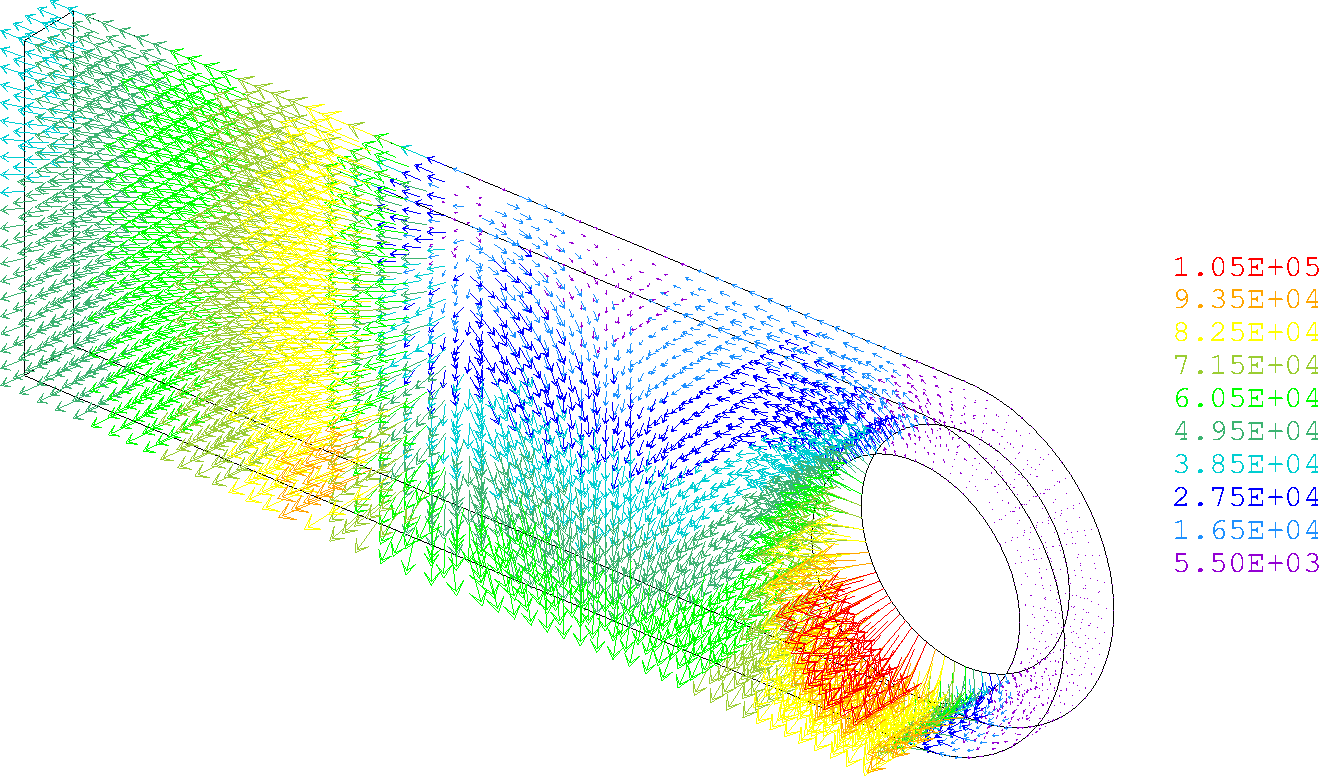
\includegraphics[height=0.5\textheight]{images/exo/4_flux}}}}
    \item<3->Ça
    \item<4->Va ?
  \end{itemize}
\end{frame}

\begin{frame}{\fe{Problème étudié}{Problem description and boundary conditions}}
  \begin{itemize}
    \footnotesize
    \item \fe{Température imposée \hspace{2cm} Flux de chaleur imposé}
             {Imposed temperature}
    \tiny
    \begin{tikzpicture}
      \node[anchor=south west,inner sep=0] (image) at (0,0)
      {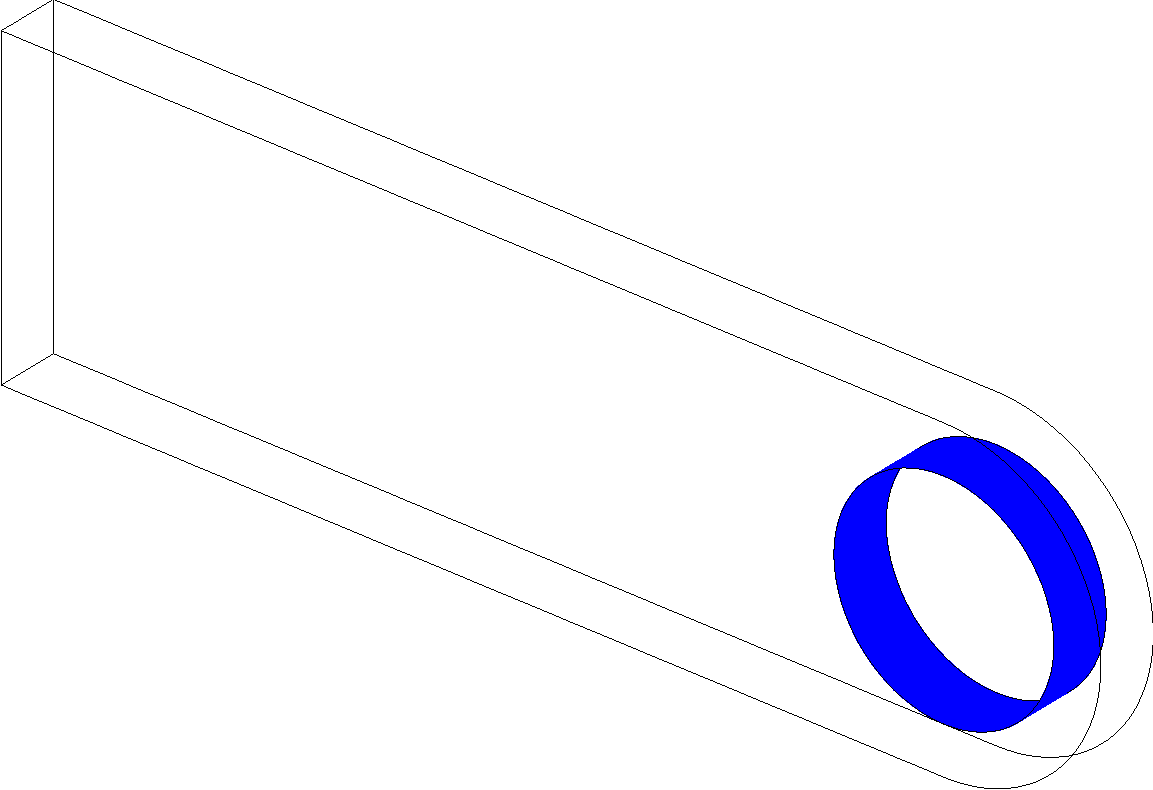
\includegraphics[width=3cm]{images/exo/2.1_cl_temperature}};
      \begin{scope}[x={(image.south east)},y={(image.north west)}]
        \draw (1,0.3) node[anchor=north west] {\blue{$T$~=~250~°C}};
      \end{scope}
    \end{tikzpicture}
    \begin{tikzpicture}
      \node[anchor=south west,inner sep=0] (image) at (0,0)
      {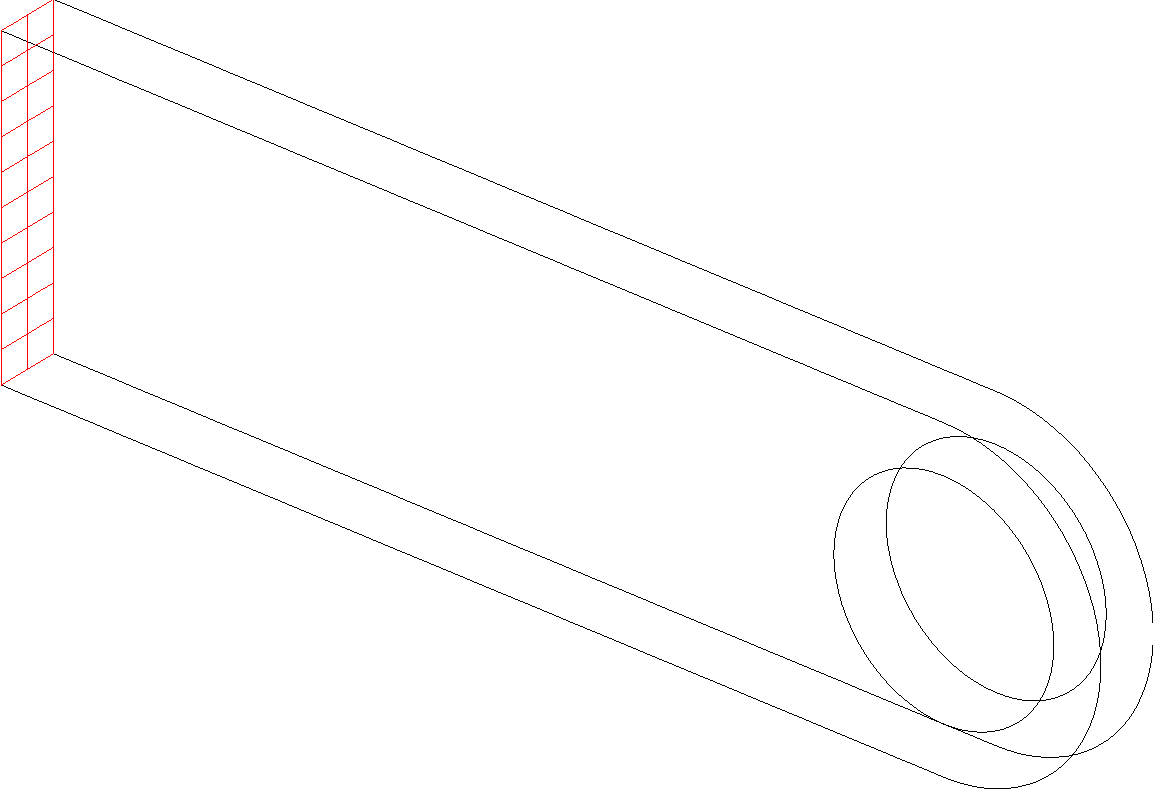
\includegraphics[width=3cm]{images/exo/2.1_cl_flux}};
      \begin{scope}[x={(image.south east)},y={(image.north west)}]
        \draw (-0.6,0.8) node[anchor=north west] {\red{$\phi$~=~-40~kW.m$^{-2}$}};
      \end{scope}
    \end{tikzpicture}
    \normalsize
  \end{itemize}
\end{frame}
